Even though a lot of visualisation tools for different use cases emerged, there is only a small amount of tools trying to animate the transition between two visualisations. This chapter provides three types of exemplarily selected tools:

\begin{enumerate}
\item tools that use some kind of animation to create the visualisation,
\item tools that also allow creating maps and
\item tools that try to animate the transition when changing the visual appearance.
\end{enumerate}

In order to evaluate all applications with the same base, the analysis framework mentioned in chapter \ref{s:basics} on page \pageref{s:basics} is used.

\subsubsection{SandDance}
\citeauthor{Drucker2015} describe a tool which makes use of so called unit visualizations. This type of visualization is best described as using one complete row of a dataset and representing it as a unit. Advantages of using units are described in the following list \iacite{Drucker2015}:
\begin{itemize}
\item \textbf{The forest and the trees:} when using a visualization based on aggregation of data, it is possible to hide outlying data or have outlying data influence the representation \iacite{Drucker2015}. However, unit visualizations maintain a one-to-one correspondence between rows in a dataset with the represenation. While classical bar charts only show one static bar for each aggregated attribute, unit visualizations show the dynamic units building that bar. Therefore, a bar for a bar chart made in a unit visualization is not a single, static shape. It is a dynamically created bar with shapes representing each unit individually and thus showing the trees yielding the forest instead of showing only the forest.

\item \textbf{Semantic constancy:} the connection between a row and a unit is maintained throughout all changes. Thus, changing visual attributes or switching from one visualization to another, does not break that bond.

\item \textbf{Direct interaction:} when using the concept of unit visualizations, it is fairly easy to show additional information of each unit by providing for example tooltips. Even when using multiple views, the concept of linking and brushing (see chapter \ref{s:linking-brushing} on page \pageref{s:linking-brushing} fore more information) can be accomplished by highlighting the selected units in every view. Furthermore, if some kind of aggregated visualization is implemented with this concept, the units can still be highlighted because they are still visible.

\item \textbf{Animation:} because of the semantic constancy, it is possible to animate smoothly between different visualizations. Transitions only update the position of every unit since they are all present.

\end{itemize}

Albeit showing a lot of advantages, the concept of unit visualizations show some weaknesses:

\begin{itemize}
\item Using a lot of units, for example, in a bar can lead to visual clutter compared to a single, static aggregated one.

\item Accessing the information of the aggregation needs more calculation in a unit visualization because each unit already represents its row and still needs to know its particular group for aggregation. First, this group needs to be calculated and second, some attributes e.g. count or sum needs to be shown in the visualization.

\item Scaling is the main weakness of this type of visualizations. Aggregate visualizations can potentially use a much larger dataset, compared to unit visualizations. Scaling does not only include the amount of data used, it also includes the hardware accessible. Displaying thousands of items and animating them requires more operation power than calculating an aggregation and drawing a rectangle on a fixed position.

\end{itemize}

\begin{figure}[!htb]
\centering
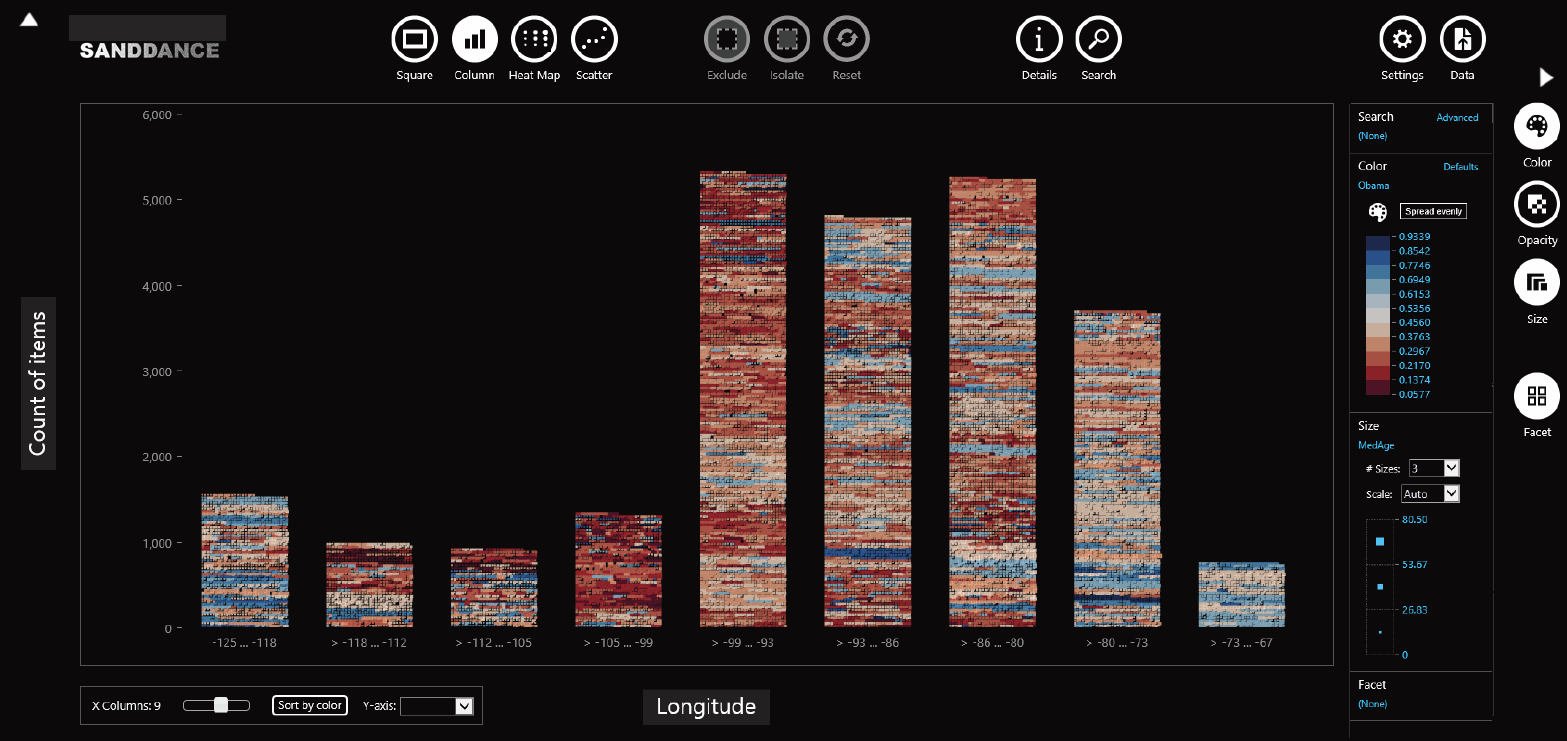
\includegraphics[width=0.8\textwidth,keepaspectratio]{images/methods/related/sanddance.png}
\caption[
    Concept of SandDance \iacite{Drucker2015}.
]{SandDance}
\label{fig:sanddance}
\end{figure}

Figure \ref{fig:sanddance} on page \pageref{fig:sanddance} shows the prototype. It allows to manually change visual channels to the right and change visual appearance e.g. changing the type of visualization at the top left. According to the analysis framework, SandDance uses static tables as input data only. \citeauthor{Drucker2015} states, that the tool was built to explore the benefits of using unit visualizations. Therefore it has no real use case to analyse, because it was used to show a completly different type of visualization without considering user benefit. However, one could say that the tool can be used to consume information and maybe discover new knowledge if using non-preexistent datasets.
SandDance can be still analysed when looking at how they implemented the visualization idiom: they freely allow users to encode attributes, even suggesting appropriate values automatically. Manipulation is implemented with a possible change in visual appearance and selection of shown data. The selection can further be filtered in different ways by either isolating or excluding data based on the given criteria.
Based on the three different types of tools already mentioned, SandDance counts as a tool supporting multiple views with different types of visualizations including maps. Furthermore it animates the transition when changing visual appearance in some kind of linear but not understandable way. Creating a new visualization is also animated with the same concept.


\subsubsection{Visual Sedimentation}
\citeauthor{Huron2013} developed a novel design metaphor inspired by the physical process of sedimentation. The design metaphor is called visual sedimentation and describes the process of aggregating falling objects due to gravity over time into static shapes \iacite{Huron2013}. This concept can be applied very well to streamed data. Incoming data items would be represented by falling objects, animated by virtual forces and aggregating over time in static shapes.
The basic concept of visual sedimentation can be described in four steps:

\begin{enumerate}
\item A new data item is processed and "enters" the scene.
\item Virtual forces are applied to the data item and suspension occurs while falling to the ground.
\item Items are accumulated on the ground or on top of previous items.
\item Items are merged into an aggregated shape.
\end{enumerate}

The possible datasets for visual sedimentation are quite obvious: all the examples discussed in the paper are some kind of dynamic, streamed data including a temporal attribute. This fact already answeres the first question of the analysis framework. Nonetheless, the concept and the examples could be extended with using static datasets without any kind of attribute of a temporal nature. Preprocessing and sorting the dataset before dropping items into the scene could yield interesting results. The weakness of using static datasets is that it stops after every item being processed. Aggregating an item into a static shape is based on multiple decisions in visual sedimentation. Thus it yields to non-aggregated data items on top of an aggregated shape when the dataset is finished. This does not happen when using streamed data.
The reason that visual sedimentation does not allow any kind of interaction leads to the answer of why even use it. It is mainly used to present some kind of data and to enjoy the visualisation itself. It is not possible to get more information on neither a single data item nor an aggregated shape.
The discussed examples are all based on two facts:
\begin{enumerate*}
\item all of them use streamed data including a temporal variable and
\item all data items have the same categorical attribute.
\end{enumerate*}
Thereby, visual sedimentation makes use of visualisations which are able to handle categorical data and use color as the visual encoding channel.

\begin{figure}[!htb]
\centering
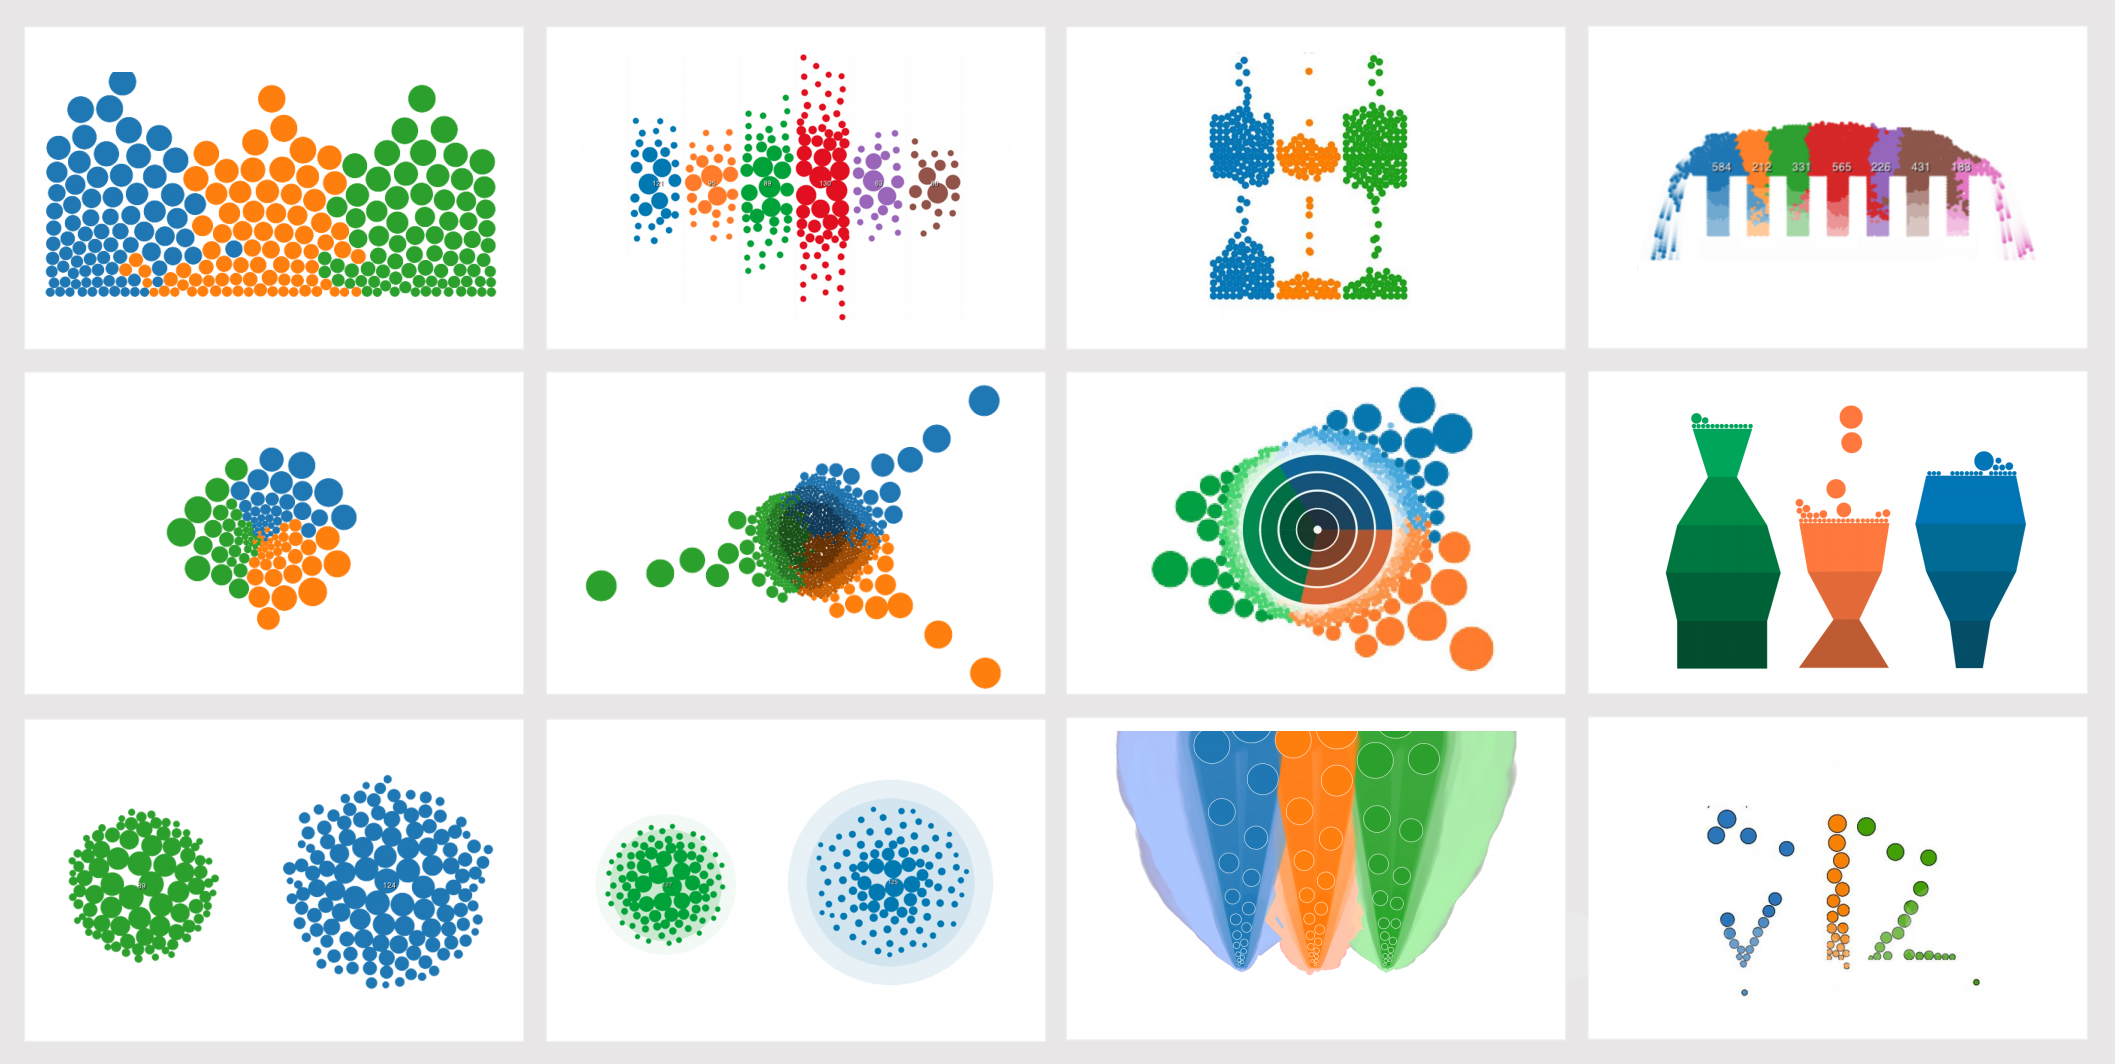
\includegraphics[height=5cm]{images/methods/related/visual-sedimentation}
\caption[
    Charts created by visual sedimentation \iacite{Huron2013}.
]{Charts created by visual sedimentation}
\label{fig:visual-sedimentation}
\end{figure}

Figure \ref{fig:visual-sedimentation} on page \pageref{fig:visual-sedimentation} shows possible charts made by visual sedimentation.

\subsubsection{FluxFlow}
\citeauthor{Zhao2014} present an interactive visual analysis system designed for revealing and analyzing anomalies spreading in social media. The main challenge of such a system is to distill valuable information from streamed social media data, due to the heterogeneous and dynamic crowd behaviours \iacite{Zhao2014}. The challenge is not further described in this thesis because it is irrelevant as related work. However, some parts of the visual analysis system are very interesting and worth a rough analysis.

Figure \ref{fig:fluxflow} on page \pageref{fig:fluxflow} shows FluxFlow. It is based on multiple views combined with linking and brushing. As one can see, it deconstructs heterogeneous social media data and builds some kind of tree. The tree can be navigated and single nodes can be highlighted with hovering. Clicking on a single node creates a new view showing all its subnodes as circles on a timeline. The radius of the circle depends on an attribute of the data item. The creation of the timeline is linear animated. Each click on a node appends a new timeline in given view.

\begin{figure}[!htb]
\centering
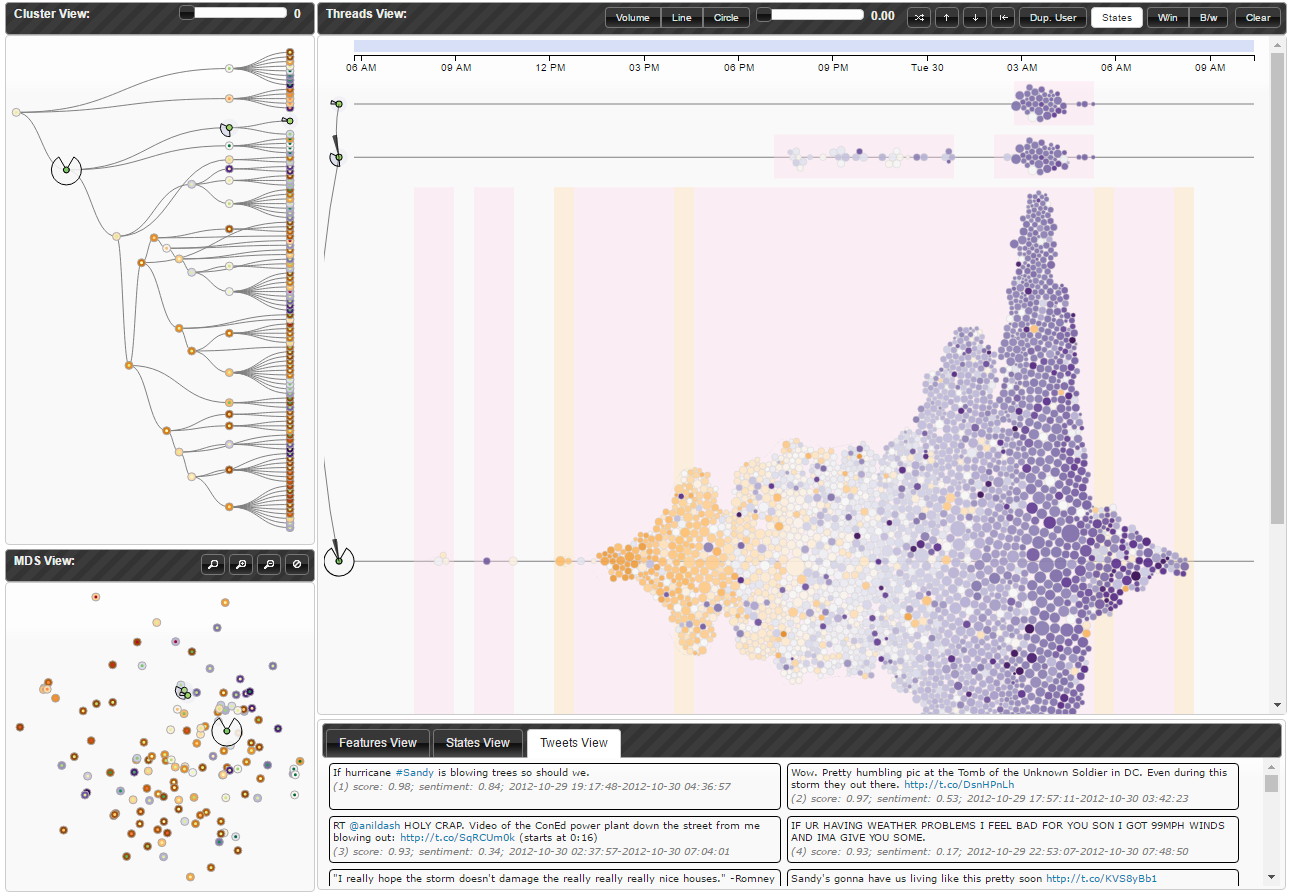
\includegraphics[height=5cm]{images/methods/related/fluxflow.png}
\caption[
    Fluxflow: a visual analysis system \iacite{Zhao2014}.
]{Fluxflow: a visual analysis system}
\label{fig:fluxflow}
\end{figure}

The use case of such a system is very well described in the paper, therefore making it easy to analyze possible datasets. Even though the main challenge of the system is to analyze streamed data, the visualisation itself is only based on static datasets. It is not clear if the system is able to build the tree from a table dataset itself or if the tree must be given.
The objective of FluxFlow is to show anomalies in social media data and discover insights with using the multiple view system combined with multiple visual channels and interaction methods. Manipulating the visualisation is possible through interaction with the timeline, selecting interesting nodes in the tree or entering specific time slots to view.

\subsubsection{Gapminder}
Gapminder\footnote{See \href{https://www.gapminder.org/}{https://www.gapminder.org/}} is very well known in the information visualisation community and the content of the data it uses is entirely explored. It shows wealth and health of countries over time and has more than 500 datasets as a basis. The default visualisation of gapminder is an extended scatter plot where the x-axis shows income per person, the y-axis life expectancy in years, the bubble itself represents the total population of each country by size and the color indicates the region of the country. Furthermore, the scatter plot is expanded with a timeline. The interactive demo of Gapminder also allows users to inspect different indicators of wealth and health.

\begin{figure}[!htb]
\centering
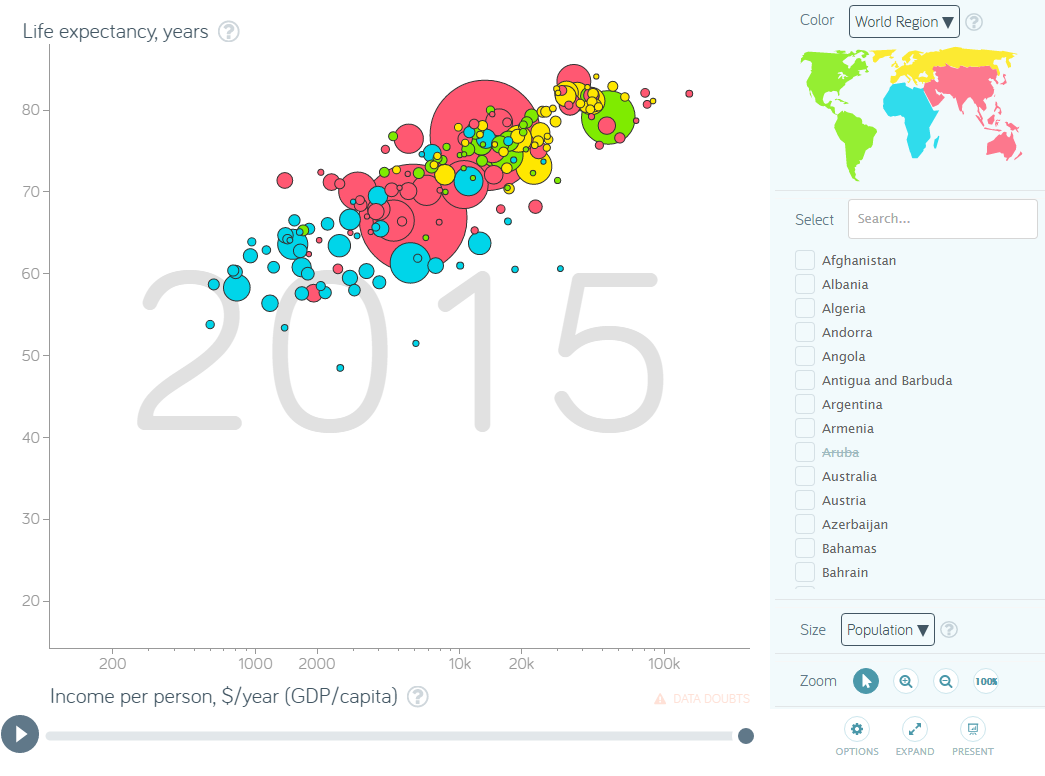
\includegraphics[height=5cm]{images/methods/related/gapminder.png}
\caption[
    Gapminder
]{Gapminder}
\label{fig:gapminder}
\end{figure}

Gapminder is not visualisation tool, but demonstrates a very popular example of animation in visualisations as a practical example. Figure \ref{fig:gapminder} on page \pageref{fig:gapminder} shows the application displaying the data corresponding to the year 1904. Users have some control over the visualisation shown:
\begin{itemize}
\item changing the attributes mapped,
\item controlling the animation by playing and pausing it directly,
\item selecting the countries which are of interest and
\item setting the symbol size.
\end{itemize}

The application made it possible to discover that people live longer in countries with a higher \ac{GDP} per capita. Countries with a low income have really short life expectancy. Furthermore, it is also discovered, that living in middle-income countries, the lifespan is huge, depending on how the income in the country is distributed and used.


\subsubsection{Tableau}
Tableau Software is an American computer software company producing a variety of data visualisation products focused on business intelligence. It offers five main products:
\begin{enumerate}
\ditem{Tableau Desktop} is used for all kinds of development. This tool is capable of creating a variety of visualisations and integrating interactions in all kinds of way depending on the visualisation.

\ditem{Tableau Server} handles shared visualisations created in Tableau Desktop.

\ditem{Tableau Online} is the same as Tableau Server except a cloud-based solution.

\ditem{Tableau Reader} allows to open shared visualisations.

\ditem{Tableau Public} combines the core components from Tableau Desktop and Tableau Server.

\end{enumerate}

The rest of this section is related to the Tableau Desktop product because it is the most interesting one. Its mission is to help people see and understand their data \iacite{Murray2013}.
Tableau offers data connections from databases, as well as simple text files and therefore can handle most kinds of dataset types. It even provides a web data connector allowing to create a connection to any kind of data accessible over HTTP. This can include internal web services, JSON data, REST APIs, and many other sources. Thus Tableau can handle static, as well as dynamic datasets.
As \citeauthor{Murray2013} already stated, Tableau wants to simplify the process of understandability and interpretability. Therefore, customers of tableau consume their information and derive knowledge. This can be done by creating multiple linked visualisations with appropriate interaction. Tableau offers concepts like detail on demand, linking and brushing, creating temporal animations, and so forth.
The most important part of Tableau Desktop is its dashboard. It is completely customizable, offering multiple methods to manipulate the given visualisation with selections, visualisation navigations and changes in visual appearances.



\subsubsection{Procedures of solution}
\label{s:theoretical-contrib}
Based on the discussed practical applications and novel visualization approaches, one can see that there is no such tool combining thematic maps with animations when changing visual appearance. The advantages and disadvantages of all aspects have been broached and discussed. This thesis will furthermore discuss and show a novel approach based on the concept of unit visualizations combined with classical thematic maps and animations when changing visual appearance. However, there are multiple possible solutions. This section will discuss some solutions with the requirement of building an an interactive web application. The solutions should yield answers to the question of which tasks can be supported by particle aggregation in thematic maps and how can the aggregation be realized.

In order to realize a practical solution for the given question, it is assumed that a dataset including heterogeneous data and some kind of geospatial data is given.

According to the mantra of \citeauthor{Shneiderman1996}, the application should start by giving an overview of the dataset. With the main concept in mind, there are two possible solutions:
\begin{enumerate}

\ditem{Unit-based grid} \hfill \\
SandDance features an approach of showing a grid as visualization, where all data items are represented as some kind of shape. Figure \ref{fig:sanddance-grid} on page \pageref{fig:sanddance-grid} shows the implementation of a unit-based grid.

\begin{figure}[!htb]
\centering
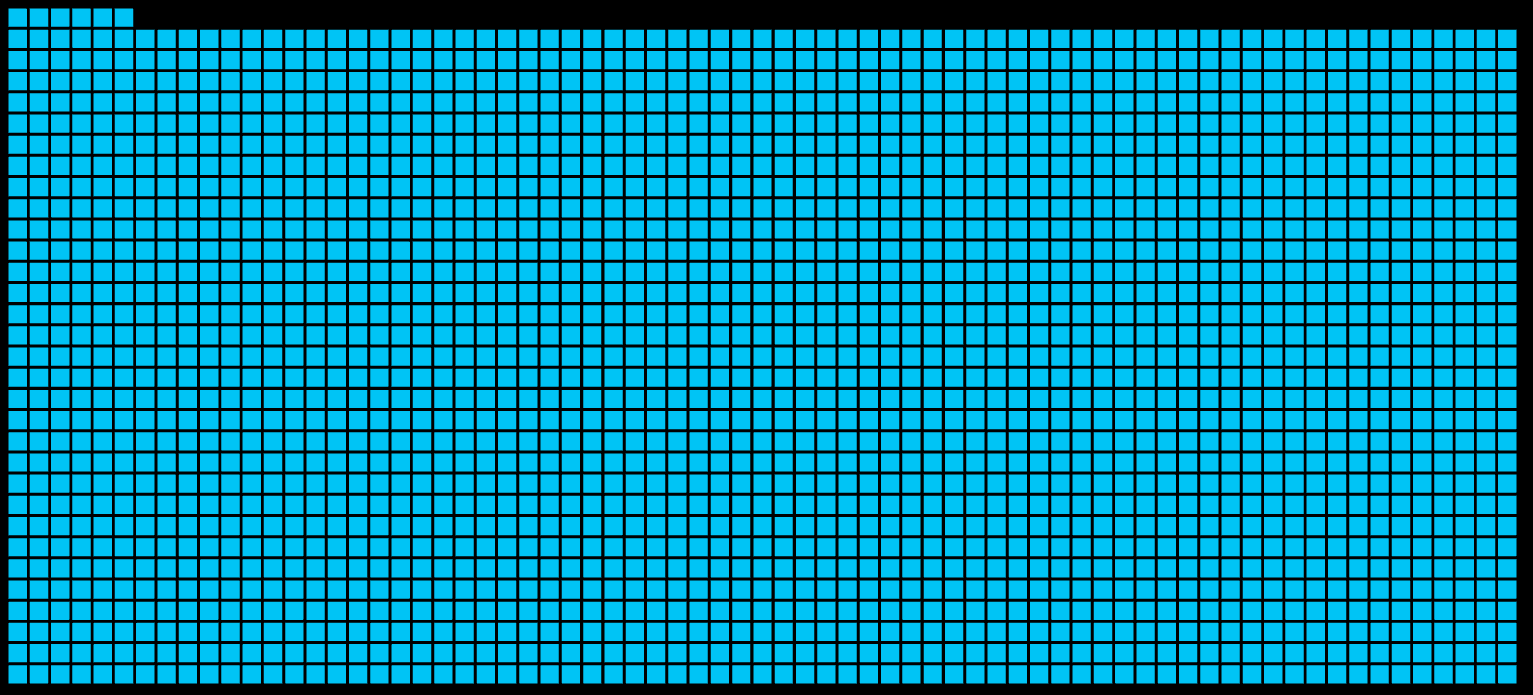
\includegraphics[height=5cm]{images/methods/related/sanddance-grid.png}
\caption[
    Unit-based grid in SandDance.
]{Unit-based grid in SandDance}
\label{fig:sanddance-grid}
\end{figure}

\ditem{Dot map} \hfill \\
Chapter \ref{s:dot} on page \pageref{s:dot} discusses the concept of dot maps in detail. This kind of thematic map can be used in combination with a one-to-one relation ship and show every item in the dataset as a single dot on the map giving an overview of the whole dataset including its geographical distribution.

\ditem{Particle attractor} \hfill \\
Figure \ref{fig:particle-attractor} on page \pageref{fig:particle-attractor} sketches the concept of showing all data items around a particle attractor.

\begin{figure}[!htb]
\centering
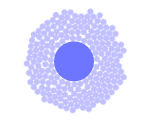
\includegraphics[height=5cm]{images/methods/related/particle-attractor.png.png}
\caption[
    Particle attractor sketch.
]{Particle attractor sketch}
\label{fig:particle-attractor}
\end{figure}

\end{enumerate}

The next step after having an overview is to decide which tasks to try out in order to test particle aggregation. One big part of this thesis already dicsusses thematic cartography in detail and thus the decision of using different types of thematic maps, which are all based on some kind of aggregation, is reasonable. Therefore trying animated particle aggregation in combination with proportional symbol maps, choropleth maps and cartograms will be a main part of the practical approach. However, there are multiple ways in changing visual appearance from an overview of the data to some kind of thematic map.

\begin{enumerate}

\ditem{In-place transition} \hfill \\
Changing from one kind of a thematic map to another one with in-place transition denotes the concept of creating the upcoming visualization. Starting with an overview grid and having a dot map as an upcoming visualization would move all particles in the same canvas to their geographical position. Having a map in the background when changing from an abstract grid to a thematic map could support the comprehensibility.
If the user determines to change the visual appearance to some other kind of thematic map, the particles would need to move according to the characteristics of the upcoming visualization. Without consideration of using other visual channels except motion, in-place transitions have multiple advantages:
\begin{itemize}
\item Semantic constancy
\item Amount of particles stays the same throughout the application (this becomes more clear when reading non in-place transitions)
\end{itemize}

\ditem{Non in-place transitions} \hfill \\
Animating the transition from one thematic map to another can also be done with an adaption of the multiple views concept. \citeauthor{Javed2012} present different visualization compositions which can be adopted for animated transitions aswell \iacite{Javed2012}:
\begin{itemize}
\item \textbf{Juxtaposition:} placing visualizations side-by-side in one view
\item \textbf{Superimposition:} overlaying two visualizations in one view
\item \textbf{Overloading:} utilizing the space of one visualization
\item \textbf{Nesting:} nesting the contents of one visualization inside another one
\end{itemize}

All of the mentioned compositions can be accomplished in two different ways. Either each particle updates its position according to the upcoming visualization, or each particle is cloned and the clone updates its position accordingly. The latter method has the major drawback of scaling poorly, because a datasize with $n$ items would need $2*n$ particles when changing the visual appearance.
\end{enumerate}

Both transition types perhaps share the same advantage: using some kind of animated transition between two different visual appearances for the same data could support the readability of the visualization. Howsoever the particles move, it could help to understand how the visualization is created and therefore could support knowledge construction.
However, starting with a particle attractor as an overview, it is also possible to use this attractor to animate the creation and transizion of visualizations. Creating marks on a visual representation could be done in two ways:

\begin{enumerate}
\item Each particle tags its spot on the map by leaving an abstract, static mark
\item Each particle moves to its spot on the map and stays
\end{enumerate}

The first method would yield animated creations, with a very basic approach when changing the visual appearance. All particles would draw upcoming visualizations every time, without considering some kind of transition from the first to the second one. The second approach can be used to initially draw the first thematic map when no other visualization is given. Changing the visual appearance if a thematic map is already shown, the mentioned transition methods can be used.

%https://imgur.com/eRDNsj3
Considering the transition from a dot map to any other type of thematic map, the aggregation needs to be animated. Figure \ref{} on page \pageref{} shows nine different ways of how particles are able to fit in or interact with a perimeter of a given abstract shape. This heavily influences the movement of particles and the readability of the map. Aggregation can not only be done by moving the particle to their new aggregated shape. It could also be accomplished by using the concept of visual sedimentation, but it would also inherit its major weakness of not showing a static when using static data. When using the concept of SandDance of building aggregated shapes with units, a map will suffer from overplotting in high density region, thus leading to visual clutter. Therefore most of the shown unit design strategies will be unusable in combination with certain thematic maps, e.g. proportional symbol maps.


\begin{table}[!htp]
\centering
\begin{tabular}{l||lllll}
& Overview & Dot Map & Proportional Symbol Map & Choropleth Map & Cartogram \\ \hline \hline
Overview &  &  &  &  \\
Dot Map &  &  &  &  \\
Proportional Symbol Map &  &  &  &  \\
Choropleth Map &  &  &  &  \\
Cartogram &  &  &  &  \\ \hline
\end{tabular}
\caption{My caption}
\label{my-label}
\end{table}
